\documentclass[10pt,a4paper]{article}
\usepackage[utf8]{inputenc}

% Define the page margin
\usepackage[margin=3cm]{geometry}

% Better typography (font rendering)
\usepackage{microtype}

% Math environments and macros
\usepackage{amsmath}
\usepackage{amsfonts}
\usepackage{amssymb}
\usepackage{amsthm}

% Define \includegraphics to include graphics
\usepackage{graphicx}

% Syntax highlighting
\usepackage{minted}

% Set global minted options
\setminted{linenos, autogobble}

% Import the comment environment for orgtbl-mode
\usepackage{comment}

% Do not indent paragraphs
\usepackage{parskip}

\title{Convex Optimization for Computer Vision, Sheet 1}
\author{Marten Lienen (03670270)}

\DeclareMathOperator{\epi}{epi}
\DeclareMathOperator{\dom}{dom}

\begin{document}

\maketitle

\section*{Exercise 1}

I will assume that $X$ in the definition of $\epi(f)$ is the domain of $f$.

\begin{proof}
  $(1) \Rightarrow (2)$: Let $(x_{1}, y_{1}), (x_{2}, y_{2}) \in \epi(f)$ and $\alpha \in [0, 1]$.
  Then $\alpha x_{1} + (1 - \alpha) x_{2} \in X$ because $\dom(f)$ is convex.
  \begin{align*}
    f\left( \alpha x_{1} + (1 - \alpha) x_{2} \right) \le \alpha f(x_{1}) + (1 - \alpha) f(x_{2}) \le \alpha y_{1} + (1 - \alpha) y_{2}
  \end{align*}
  So $\alpha \begin{pmatrix}x_{1}\\y_{1}\end{pmatrix} + (1 - \alpha) \begin{pmatrix}x_{2}\\y_{2}\end{pmatrix} \in \epi(f)$ and therefore $\epi(f)$ is convex.

  $(1) \Leftarrow (2)$: For every $x_{1}, x_{2} \in X = \dom(f)$ there are $y_{1}, y_{2}$ such that $(x_{1}, y_{1}), (x_{2}, y_{2}) \in \epi(f)$ because $x_{1}, x_{2} \in \dom(f)$.
  Because $\epi(f)$ is convex, for any $\alpha \in [0, 1]$ we have $\alpha \begin{pmatrix}x_{1}\\y_{1}\end{pmatrix} + (1 - \alpha) \begin{pmatrix}x_{2}\\y_{2}\end{pmatrix} \in \epi(f)$ and therefore $\alpha x_{1} + (1 - \alpha) x_{2} \in X$.
  So $X = \dom(f)$ is convex.

  Now let $x_{1}, x_{2} \in X$ and $\alpha \in [0, 1]$.
  Since $(x_{1}, f(x_{1})), (x_{2}, f(x_{2})) \in \epi(f)$, we have $\alpha \begin{pmatrix}x_{1}\\f(x_{1})\end{pmatrix} + (1 - \alpha) \begin{pmatrix}x_{2}\\f(x_{2})\end{pmatrix} \in \epi(f)$.
  So by the definition of the epigraph
  \begin{equation*}
    f(\alpha x_{1} + (1 - \alpha) x_{2}) \le \alpha f(x_{1}) + (1 - \alpha) f(x_{2})
  \end{equation*}
  and $f$ is convex.
\end{proof}

\section*{Exercise 2}

\begin{proof}
  Let $(x_{1}, t_{1}), (x_{2}, t_{2}) \in \dom(f)$ and $\alpha \in [0, 1]$.
  Then $t_{1}, t_{2} > 0$ and $\frac{x_{1}}{t_{1}}, \frac{x_{2}}{t_{2}} \in \dom(g)$.
  Therefore $\alpha t_{1} + (1 - \alpha) t_{2} > 0$ as well as $\frac{\alpha x_{1} + (1 - \alpha) x_{2}}{\alpha t_{1} + (1 - \alpha) t_{2}} \in \dom(g)$ because
  \begin{align*}
    \frac{\alpha x_{1} + (1 - \alpha) x_{2}}{\alpha t_{1} + (1 - \alpha) t_{2}} & = \frac{\alpha}{\alpha t_{1} + (1 - \alpha) t_{2}} x_{1} + \frac{1 - \alpha}{\alpha t_{1} + (1 - \alpha) t_{2}} x_{2}\\
                                                                                & = \frac{\alpha t_{1}}{\alpha t_{1} + (1 - \alpha) t_{2}} \frac{x_{1}}{t_{1}} + \frac{(1 - \alpha)t_{2}}{\alpha t_{1} + (1 - \alpha) t_{2}} \frac{x_{2}}{t_{2}}\\
                                                                                & = \beta \frac{x_{1}}{t_{1}} + (1 - \beta) \frac{x_{2}}{t_{2}} \in \dom(g) \qquad \textrm{with $\beta = \frac{\alpha t_{1}}{\alpha t_{1} + (1 - \alpha) t_{2}}$}
  \end{align*}
  where $\beta \in [0, 1]$ since the denominator is always greater than or equal to the numerator.
  So $\dom(f)$ is convex.

  \begin{align*}
    f(\alpha x_{1} + (1 - \alpha)x_{2}, \alpha t_{1} + (1 - \alpha)t_{2}) & = (\alpha t_{1} + (1 - \alpha)t_{2}) g\left( \frac{\alpha x_{1} + (1 - \alpha)x_{2}}{\alpha t_{1} + (1 - \alpha)t_{2}} \right)\\
                                                                          & \le (\alpha t_{1} + (1 - \alpha)t_{2}) \left( \beta g\left( \frac{x_{1}}{t_{1}} \right) + (1 - \beta) g\left( \frac{x_{2}}{t_{2}} \right) \right)\\
                                                                          & = (\alpha t_{1} + (1 - \alpha)t_{2}) \left( \frac{\alpha t_{1}}{\alpha t_{1} + (1 - \alpha) t_{2}} g\left( \frac{x_{1}}{t_{1}} \right) + \frac{(1 - \alpha) t_{2}}{\alpha t_{1} + (1 - \alpha) t_{2}} g\left( \frac{x_{2}}{t_{2}} \right) \right)\\
                                                                          & = \alpha t_{1} g\left( \frac{x_{1}}{t_{1}} \right) + (1 - \alpha) t_{2} g\left( \frac{x_{2}}{t_{2}} \right)\\
                                                                          & = \alpha f(x_{1}, t_{1}) + (1 - \alpha) f(x_{2}, t_{2})
  \end{align*}
  So $f$ is convex.
\end{proof}

\section*{Exercise 3}

\begin{proof}
  $(1) \Rightarrow (2)$: $X$ is closed, so $\bar{X}$ is open.
  Let $(x_{i})_{i \in \mathbb{N}}$ be a convergent series in $X$ with limit $x'$.
  Assume that $x' \not\in X$.
  Then there is an $\varepsilon$-ball around $x'$ that is complete contained in $\bar{X}$.
  Therefore none of the $x_{i}$ can be closer to $x'$ than $\varepsilon$ which contradicts the assumption that $\lim_{i \rightarrow \infty} x_{i} = x'$.
  So $x' \in X$.

  $(1) \Leftarrow (2)$: Let $x' \in \bar{X}$.
  Assume that there is no $\varepsilon$ such that $B_{\varepsilon}(x') \cap X = \emptyset$.
  So for every $i \in \mathbb{N}$ there is an $x_{i} \in X$ such that $d(x', x) < \frac{1}{i}$.
  These $(x_{i})$ form a convergent series in $X$ with limit point $x'$.
  But $x' \not\in X$ which contradicts the assumption that every convergent series attains its limit in $X$.
  So $\bar{X}$ is open and $X$ is closed.
\end{proof}

\section*{Exercise 4}

\begin{proof}
  $(1) \Rightarrow (2)$: Let $x \in X$, $v \in \mathbb{R}^{n}$.
  \begin{align*}
    v^{T}H_{f}(x)v & = \lim_{t \rightarrow 0} 2 \frac{f(x + tv) - f(x) - tv^{T} \nabla f(x)}{t^{2}}\\
            & \ge \lim_{t \rightarrow 0} 2 \frac{(tv)^{T}\nabla f(x) - tv^{T} \nabla f(x)}{t^{2}} = 0 \qquad \textit{apply the hint with $y = x + tv$}\\
  \end{align*}
  So $H_{f}(x)$ is positive semidefinite.

  $(1) \Leftarrow (2)$: Let $x, y \in X$.
  \begin{equation*}
    f(x + (y - x)) = f(x) + (y - x)^{T} \nabla f(x) + \frac{1}{2} (y - x)^{T} H_{f}(x + t(y - x)) (y - x)^{T} \ge f(x) + (y - x)^{T} \nabla f(x)
  \end{equation*}
  So
  \begin{equation*}
    f(y) - f(x) \ge (y - x)^{T} \nabla f(x)
  \end{equation*}
  what proves that $f$ is convex according to the hint.
\end{proof}

\section*{Exercise 5}

\begin{proof}
  \begin{align*}
    \frac{\partial f}{\partial x_{i}} = \frac{1}{2}\left( \sum_{j = 1}^{n} a_{ij} x_{j} + a_{ji} x_{j} \right) + b_{i} = \frac{1}{2}x^{T}\left( A_{:,i} + A_{i,:}^{T} \right) + b_{i} \Rightarrow f'(x) = \frac{1}{2}x^{T}(A + A^{T}) + b^{T}
  \end{align*}
  \begin{align*}
    \frac{\partial f}{\partial x_{i} \partial x_{j}} = \frac{1}{2} \left( A_{ji} + A_{ij} \right) \Rightarrow f''(x) = \frac{1}{2} \left( A + A^{T} \right)
  \end{align*}

  So the Hessian of $f$ is
  \begin{equation*}
    f''(x) = \frac{1}{2}\left(A + A^{T}\right)
  \end{equation*}
  which is still positive semidefinite:
  Let $v \in \mathbb{R}^{n}$.
  \begin{equation*}
    \frac{1}{2}v^{T}(A + A^{T})v = \frac{1}{2} \left(v^{T}Av + v^{T}A^{T}v\right) = \frac{1}{2} \left(v^{T}Av + (v^{T}Av)^{T}\right) \ge 0
  \end{equation*}
  So $f$ is convex according to exercise 4.
\end{proof}

\section*{Exercise 6}

If we understand the mask $I$ as a matrix that is $1$ for pixels that should be kept and $0$ everywhere else, we can write $u$ as $(1 - I)\bar{u} + If$ for vectorized $\bar{u}$ and $f$.

Let $\nabla_{c}$ be the gradient constructed on sheet 0.
Then you can rewrite the objective to
\begin{equation*}
  \min_{u \in \mathbb{R}^{n \times m}} ||\nabla_{c} u||_{F}^{2} \quad \text{s.t.}~u_{i,j} = f_{i,j}~\forall (i,j) \in I
\end{equation*}
Next we plug in the decomposition and drop the constraint.
\begin{equation*}
  \min_{\bar{u} \in \mathbb{R}^{n \times m}} ||\nabla_{c} \left( (1 - I)\bar{u} - If \right)||_{F}^{2} = \min_{\bar{u} \in \mathbb{R}^{n \times m}} ||\left( \nabla_{c} (1 - I) \right)\bar{u} - \left( \nabla_{c}I \right)f||_{F}^{2}
\end{equation*}
This in turn is the approximate solution of
\begin{equation*}
  \left( \nabla_{c} (1 - I) \right)\bar{u} = \left( \nabla_{c}I \right)
\end{equation*}
Finally we construct the solution by plugging $\bar{u}$ into $u = (1 - I)\bar{u} + If$ and get the result in figure \ref{fig:inpainted}.

\begin{figure}[h]
  \centering
  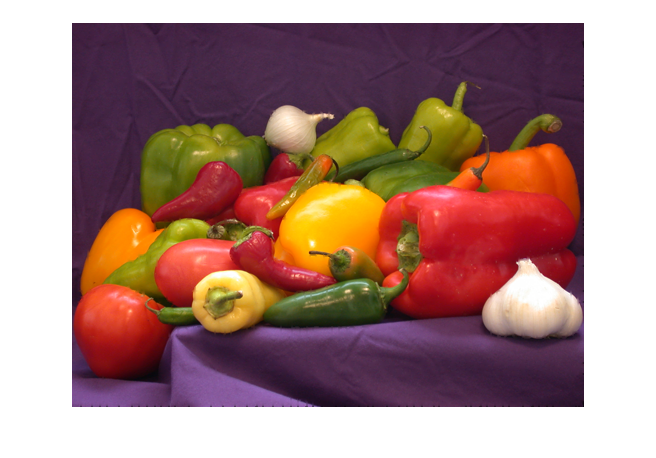
\includegraphics[width=\textwidth]{sheet-1/inpainted}
  \caption{The inpainted vegetable picture}
  \label{fig:inpainted}
\end{figure}

\begin{minted}{matlab}
  % Read image and mask
  f = imread('corrupted.png');
  nm = size(f);
  n = nm(1);
  m = nm(2);
  f = f(:);
  mask = imread('mask.png');
  mask = mask(:) > 0;
  invmask = ~mask;

  % Construct the gradient
  en = ones(n, 1);
  em = ones(m, 1);
  Dx = spdiags([-1 * em, em], [0, -1], m, m);
  Dy = spdiags([-1 * en, en], [0, 1], n, n);
  DX = kron(Dx', speye(n));
  DY = kron(speye(m), Dy);
  nablac = cat(1, kron(eye(3), DX), kron(eye(3), DY));

  % Split the gradient
  nablau = nablac;
  nablau(:, mask) = 0;
  nablaf = nablac;
  nablaf(:, invmask) = 0;

  % Construct right hand side
  b = -nablaf * double(f);

  % Solve for u-bar
  u = nablau \ b;

  % Insert into image
  f(invmask) = u(invmask);

  % Display
  imshow(reshape(f, n, m, 3));
\end{minted}

\end{document}
